\chapter{System architecture}
\label{chap:implementation}

Trust and reputation systems rely heavily on the records of interactions. Our theoretical analysis from
the previous chapter has further shown that dissemination of those records is required to ensure their
validity and therefore the validity of the trust that is built on them. In previous work our 
research group has created a tamper-proof recording system for interactions, TrustChain. This system is 
implemented in a peer-to-peer video streaming service Tribler and the IPv8 project\footnote{https://github.com/tribler/py-ipv8}.
% Although the exchange of information is part of those systems and as shown key to their manipulation
% resistance, exchanges are not explicitly recorded. 
With respect to our model though, TrustChain is limited in its ability to ensure gossiping because information
exchange is not recorded.
As such, the model of Chapter \ref{chap:model}
cannot be realized in their architecture. We created an extension of TrustChain that allows for the 
recording and reasoning about gossip behavior of agents.

We open this chapter by relating the previously introduced model to an application context. Next we
introduce the conceptual working of blockchains which is a core technology for TrustChain. A discussion of
TrustChain itself follows. Then our extension, the recording of exchanges, is discussed in detail. 
Finally, a more elaborate analysis of possible attacks on the system is performed.

\section{Relating Tribler to the ordered encounter model}
In the previous chapter the ordered encounter model was introduced. The model is useful for studying 
the mechanisms of a trust system in a theoretical 
setting. However it may not be immediately obvious to the reader how the model relates to a digital
trust system in an application context. In this section we shed more light on how the model's concepts 
match their counterparts in the Tribler application.

We introduced Tribler in Chapter \ref{chap:introduction}. It is a peer-to-peer video streaming 
service which is based on the BitTorrent protocol. As the BitTorrent protocol does not guarantee the
privacy of users, Tribler adds an onion routing layer on top of the protocol. This routing protocol 
is similar to the Tor network and ensures that traffic is encrypted and relayed multiple times before exiting the
Tribler network and entering the public internet. The origin of the original request is made anonymous.

\subsection{Agents}
In the model, agents are the entities that take part in interactions and encounters. Intuitively one
would assume that users are the agents in Tribler. It would be more accurate though to say that a 
running instance of the Tribler software is the agent. A single human user can have multiple 
instances of the software running on multiple machines and thus ``control'' multiple agents. Despite
being able to run or stop the agents, the human user has only a very small decision space, though, 
because the software runs on its own and executes according to design. 

The distinction of honest and dishonest agents is then made as follows: honest agents are the 
instances that run the software as intended while dishonest agents are instances of manipulated 
software. 

Each running instance of the Tribler software can be uniquely identified. It makes use of asymmetric
cryptography for authentication and encryption. Specifically, Curve25519 is used in an 
elliptic curve Diffie-Hellman key agreement scheme. 

In the following description of the system we will use both, ``node'' and ``agent'' when referring to the 
behavior of a Tribler instance executing some action. 

\subsection{Interactions}
The interactions that we defined in the ordered interaction model map very well to the transactions
of data in Tribler. Peer-to-peer video streaming in Tribler works through uploading and downloading 
portions of data from any agent in the Tribler network based on the BitTorrent protocol. Also, as
mentioned above, agents relay traffic in the Tribler network for peers. Relaying again can be seen 
as a similar transaction where the incoming data is downloaded and immediately uploaded to the next
agent in the routing scheme. These transactions of data map to the transactions in our model and 
need to be recorded in a tamper-proof manner. For this recording of transaction Tribler implements 
TrustChain, which is discussed in 
more detail in Section~\ref{sec:trustchain}. The discussion of how to create those records, secure 
them against manipulations and distribute them in the network is the centerpiece of this work.

\subsection{Trust and reputation}
The uploading and downloading of videos in the network is a social dilemma as each user wants to 
stream videos while contributing as little as possible. It is therefore a good test bed for a trust 
system which should incentivize users to contribute. The reputation of an agent in Tribler represents the 
contribution behavior of that agent. Contributing, that is uploading video streams to other users,
increases an agent's reputation whereas downloading, that is streaming videos, decreases an agent's 
reputation. Also, relaying is a neutral activity in terms of the upload-download ratio, yet the 
reputation of an agent that relays a lot of data needs to be higher as well. In contrast to 
reputation, trust is subjective and can be seen as the subjective perception of a peer being a 
``good contributor''. 

In order to better illustrate the difference between reputation and trust we provide an example.
Assume an agent $A$ knows two agents, $B$ and $C$ and sees that both have uploaded and downloaded 
the same amount of data. However, $B$ has uploaded most to $A$ while $C$ has uploaded only to 
agents that $A$ has not heard of. Human intuition tells us that $A$ should trust $B$ more than $C$, 
because of the stronger direct connection. Trust therefore depends on the topography of the network.

% % 
% % Is this necessary??? 
% \section{Reciprocity}
% % 

\subsection{Exchanges}
As we have shown in Chapter \ref{chap:model}, the exchange of information is a major component of a trust 
systems defense against manipulators and free-riders. Yet, TrustChain does not create records on 
gossip. We identify this as a limitation. 

Honest Tribler agents actually do exchange data in order to calculate a non-zero reputation for possible
future peers. Still, without recording of this behavior, it cannot be rewarded or its absence be punished. 
This is why we propose an extended TrustChain which enables recording of gossip and gossip-about-gossip. 
The details of this extension are discussed in Section \ref{sec:extension}.

\section{Blockchain basics}
The design of distributed databases bears many challenges. Especially if sensitive data is involved
and users need to have access globally, the asynchrony of events, lack of guarantees on data 
consistency and agent honesty create issues. For the early years of the internet those challenges seemed
insurmountable. That is why most services that act on sensitive data are centralized, examples being 
banks, government institutions or commercial services like Facebook\footnote{https://facebook.com}.
Centralization has its own shortcomings such as abuse of power, dishonesty, single point-of-failure
and platform lock-in. We described those issues in more detail in Chapter \ref{chap:introduction}.
The increasing significance of those issues led to the design and implementation of the Bitcoin 
protocol~\cite{nakamoto2008bitcoin} for digital money transfers. The Bitcoin protocol allows a distributed network of agents 
to agree on the exact order of events, through a hash chain which acts as a distributed timestamp 
server and the proof-of-work algorithm. This architecture is commonly referred to as Blockchain. We
shall introduce this concept in more detail as the core concepts are also applied in TrustChain.

\subsection{Concept}
A blockchain is essentially an append-only database in form of chained blocks. It is designed to be
used as a secure information storage in distributed systems without any central governance. Tribler
is therefore a possible application context for a blockchain-based database.

Each block on the chain contains a set of transactions, the root hash of that set, a Nonce (used in 
the consensus algorithm) and the hash of the previous block. Through the hash of the previous block the blocks are 
chained together as can be seen in Figure~\ref{fig:basic_blockchain}. The first block in the chain 
is called the genesis block. The Bitcoin blockchain and similar single-chain blockchains only has 
one genesis block. Each block can also be identified by a sequence number, which is an increasing 
integer that starts from 1 at the genesis block.

Transactions and new blocks need to be published publicly on the network. The block creation process
is managed by the consensus mechanism Proof-of-work. This process is also called mining and the nodes
that take part in it are thus miners. It works as follows: Each new block contains a computational 
intensive puzzle which needs to be solved in order to be able to publish a block. A string needs to 
be found that matches a target hash. All miners use their CPU to guess the correct string. Once they
find a possible solution, the agent combines all the transactions that were published since the last
block and combines them to a new block. The block size is fixed such that after adding a certain number of 
transactions the block is considered complete. Once complete, the agent publishes the
block on the network. Any agent that receives the block will verify that
the solution to the puzzle is correct and all transactions are valid. If so, they add the new block
to their copy of the chain and start with solving the next puzzle in order to become the next 
creator of a block. The creator of the block is rewarded with newly created Bitcoins.

\begin{figure}
    \centering
    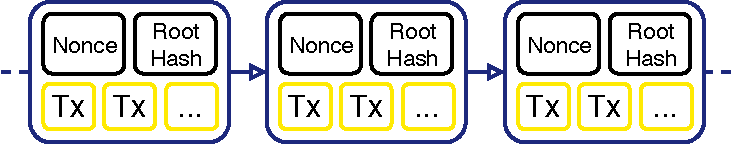
\includegraphics[width=0.7\textwidth]{images/blockchain.pdf}
    \caption{Conceptual depiction of a slice of a Bitcoin-like blockchain. Blocks contain multiple transactions and are chained together through the hash of the previous block. Source: \textit{Creation of TU Delft BLockchain Lab}}
    \label{fig:basic_blockchain}
\end{figure}

All agents are acting on the same copy of the blockchain. The one global chain therefore contains 
all transactions that happen on the network. This implies that all agents need to be informed about any new block.
In order to allow for enough time to synchronize transactions and blocks, the difficulty of the puzzle 
can be increased. This ensures a approximately fixed time between new blocks. This block time is 
10 minutes for Bitcoin. Together with the fixed block size the global transaction throughput of the
system is capped. For Bitcoin this is approximately 7 transactions per second. The Bitcoin solution
does not scale and is in its current state no possible solution for a global trust system.

\subsection{Consensus}
% why?: 
Bitcoin-like distributed ledgers create an incentive for agents to publish new blocks by rewarding 
them with currency. New blocks are accepted if they are on top of the longest chain. This creates 
an incentive for all participating miners to stay up to date on the state of the global ledger. Only
if an agent is in possession of the latest block is there a chance to receive the block reward. 

Conflicts can arise when two blocks are found at approximately the same time. Each block will be 
considered the latest by part of the network. The network is thus split into two groups and a natural
fork is created in the chain. However this conflict will usually resolve itself. Both parts of the 
network will continue to mine the next block. Depending on the CPU power of the two groups and some
luck, one group will be faster at mining the next blocks. Because blocks are only rewarded when they
have the highest sequence number, the slower part of the network will quickly switch to the longer
chain and thus the network is combined again. 

Bitcoin thus guarantees that all agents have the exact same chain of blocks(except for the latest 
blocks) and thus have a single view of the state of each agent. This state of agreement is called
global consensus.

\subsection{Tamper-proof}
% why?: show that the hash chain creates a tamper-proof record
The chain of hashes that connects blocks on the blockchain creates a tamper-proof history. Any 
change to a block on the chain will change the hash of that block. This voids the following block's
hash pointer because it points to the old block. Therefore any change to the block requires the 
recalculation of all following blocks. Because all blocks need to be agreed upon on the network 
other agents will be able to see such tampering with the blocks and will not agree on it. 

The tamper-proof nature of the blockchain makes it a very useful tool for recording chronologically 
ordered transactions. The sequence of blocks also orders the transactions stored in the blocks. Any
transactions in an earlier block happen before the transactions in the later block. Also, as was just 
explained, any change to the ordering of transactions will result in a break in the hash chain. Even though this order
does not necessarily correspond to the local time of the agent who published the transaction, the 
blockchain will create a globally accepted order for transactions.  This is a major 
achievement because this order is robust against network delays, tampering and other attacks.

Still the system cannot be perfectly secure. One way to actually attack the system is by mining 
blocks faster than the rest of the network. This is only possible when a majority of the network's 
CPU power works together which is unlikely for very large networks. Yet, there are examples of this 
happening~\cite{51percentbitcoingold, 51percentverge}.

\subsection{Scalability}
A blockchain solution like Bitcoin seems like a valid implementation for the ordered encounter model that we defined in the 
previous chapter. All transactions are exchanged with all agents on the network. The blockchain 
creates a totally ordered set of all global transactions which intrinsically means that each agent's 
transactions are also fully ordered. Double spend and forks are detectable through global consensus. 

However, the Proof-of-work mechanism leads to issues in scalability. The global throughput of 7 
transactions per second is not enough to power a global scale distributed trust system as we envision it. 
The Proof-of-work consensus algorithm also leads a to a large expenditure of energy which creates 
large transaction costs. This is not acceptable if the trust system should be for general purpose 
applications. For example, users will not accept to pay for each video they stream on the Tribler 
platform. A different solution is therefore needed.

\section{TrustChain}
\label{sec:trustchain}
TrustChain is designed with scalability in mind. It's design focus is in stark contrast with that of
Bitcoin. Instead of employing global consensus to guarantee a single global transaction set, 
all agents in the TrustChain fabric are owner of a chain for themselves. This creates a scalable 
solution in which the total network throughput grows with the size of the network. However, the
scalability comes at the cost of security guarantees. This section will first discuss the general 
architecture of trust chain before discussing the scalability and some details of the implementation.

\begin{figure}
    \centering
    \begin{subfigure}{0.49\textwidth}
        \centering
        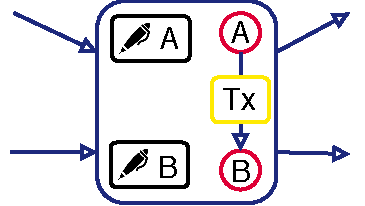
\includegraphics[width=0.8\textwidth]{images/block-2.pdf}
        \caption{Conceptual representation}
    \end{subfigure}
    \begin{subfigure}{0.49\textwidth}
        \centering
        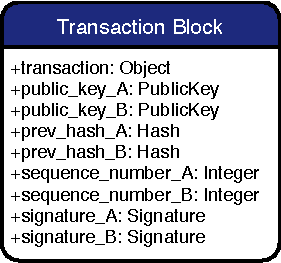
\includegraphics[width=0.6\textwidth]{images/transaction_block_data.pdf}
        \caption{Transaction block, data representation}
    \end{subfigure}
    \caption{A single block in the TrustChain fabric. Incoming arrows represent block hashes from the previous blocks of the agents' chains. Source: \textit{Creation of TU Delft BLockchain Lab}}
    \label{fig:trustchain_block}
\end{figure}

\subsection{Data structure}
\label{sec:transaction_blocks}
Similar to the Blockchain architecture TrustChain records transactions in blocks and links blocks 
with the use of hash pointers. Though, in contrast to having a single chain of blocks for the whole
network, in TrustChain each agent starts with an own genesis block. Hence, all agents record their
own transactions on their own chain. 

Blocks in TrustChain record exactly one transaction between two parties. Because both parties have 
their own chain and the transaction concerns both parties, any new block is added to both agents'
chains. Each block contains the following main elements:

\begin{itemize}
    \item \textbf{Transaction.} The transaction field records the value that was exchanged between agents.
    TrustChain is designed to be application agnostic. Thus the content of a transaction can be any 
    serializable data. 
    \item \textbf{Previous block hashes.} The hashes of the previous blocks of both agents' chains 
    firmly attaches the new block to their history. This is similar to the basic blockchain concept.
    \item \textbf{Public Keys.} In order to uniquely identify the two agents that conduct a transaction
    their public keys are recorded.
    \item \textbf{Signatures.} Both agents provide a digital signature of the transaction with their 
    private key which any agent can check with the agents' public keys. This authenticates the 
    transaction and cryptographically proves that the real owners of the private key conducted the 
    transactions.
    \item \textbf{Sequence numbers.} All blocks on an agent's chain have a unique sequence number 
    which shows the position in the chain. 
\end{itemize}

A simplified depiction and data representation of a TrustChain block is shown in Figure~\ref{fig:trustchain_block}. When 
looking at a single agent the given data structure creates a chain of blocks which describes all the
transactions of that agent. However the second incoming and outgoing edge of each block entangles an
agent's chain with those of all partners. When looking at a complete network, of the transactions the
represents a directed acyclic graph(DAG). Such a structure is shown in Figure~\ref{fig:trustchain_graph}.

\begin{figure}
    \centering
    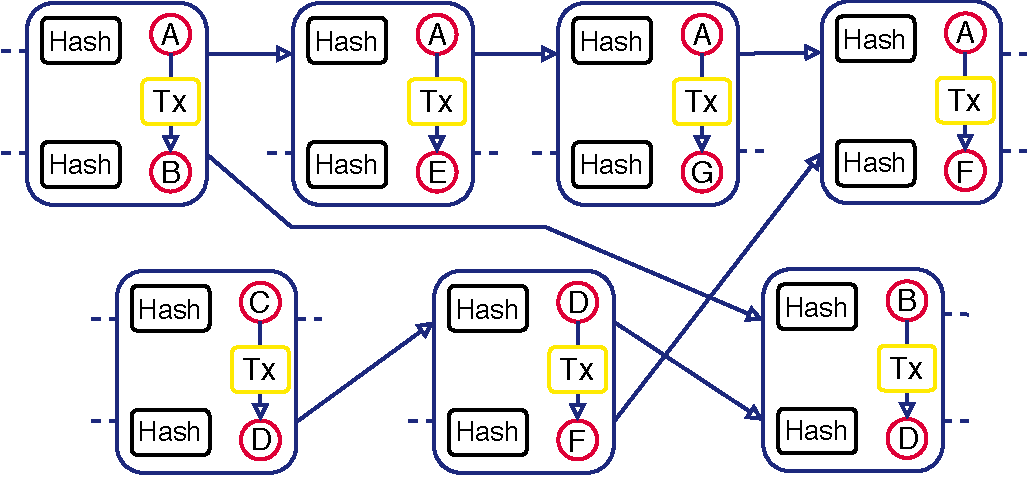
\includegraphics[width=\textwidth]{images/trustchain_graph.pdf}
    \caption{TrustChain graph structure with multiple transactions. The top row shows the chain of
    an agent A with links to multiple other blocks. Source: \textit{Creation of TU Delft BLockchain Lab}}
    \label{fig:trustchain_graph}
\end{figure}

The validity of a block depends on the following conditions. 

\begin{itemize}
    \item the transaction field contains the necessary information to properly define a transaction in the application context. For Tribler this
means that it needs to contain at least the amount of data which was uploaded and downloaded between
the two agents. 
    \item both block hashes need to point to the valid, previous block on the chain of the same public key. This makes the validity a recursive definition 
which depends on the previous content of the chain of both agents.
    \item both public keys need to be valid public keys
    \item the signatures need to be correct for the given public keys and block content
    \item the block needs to carry the next integer as sequence number compared to the blocks that the previous hashes point to
\end{itemize}

Any agent is able to confirm the validity of a block given the full chains of both agents up to the 
block that is to be verified. We consider next the impact of this architecture on scalability and
security.

\subsection{Scalability}
\label{sec:trustchain_scalability}
For a transaction to be successful in TrustChain, only two agents need to agree on the content. This
means that only two agents need to communicate to confirm a transaction. Transactions do not need to 
be publicly announced or sent to all nodes on
the network. Also, multiple transactions can be performed at the same time globally without breaking
the rules of the system. In contrast to the Bitcoin system, only the transactions of each agent are
strictly ordered, the global set of transactions is not.

This result is a system that scales with the size of the network. A simple example makes this very 
clear. Consider two networks, one with 10 nodes and one with 100 nodes. For simplicity we consider
time to be discrete and agents to interact in rounds. Each transaction takes 1 round and all agents 
interact. Throughput calculation is then straightforward. Nodes arrange in pairs and perform a
transaction. The small network will have 5 pairs and thus 5 transactions per round, while the large
network has 50 pairs and transactions. Although this example is extremely simplified, no real-world
effect like network delays, network churn or bandwidth restrictions greatly conflict with this property.

TrustChain does not include a global consensus and thus does not expend bandwidth, storage and 
computational power to create a global order for transactions. That removes the most costly component
from the general blockchain architecture. Without the expense of CPU power for solving an inverse 
hash problem, transactions only cost the bandwidth and computational expense of communicating with 
the direct interaction partners. TrustChain enables free transactions in a global distributed 
system with scaling throughput based on the network size. Hence, TrustChain is valid solution for a
global trust system.

\subsection{Security}
The scalability of the TrustChain architecture comes at the expense of some security guarantees.

Similar to a single Blockchain the graph structure of TrustChain creates a tamper-proof record of
transactions. A large difference is that each agent reigns over a chain. Each agent seemingly is 
able to reorder transactions but blocks are signed by a second agent and the signature will become
invalid if the blocks are tampered with. Also blocks contain the previous hash of the counter party's
previous block. That ensures that the hashes cannot change without the other agent being able to 
detect the tampering.Therefore transactions are still recorded in a tamper-proof data structure.

Still, detectabillity does not ensure detection. The can only be secured if agents
continuously verify their partners data. Also, as the validity of a block is recursively defined, 
agents can only ensure the validity of a partners previous transaction if they possess their complete
chain and verified that chain. It is even harder to defend against attacks in which agent do not 
directly manipulate the data structure but make use of the incomplete knowledge which is intrinsic 
to distributed networks. In Section \ref{sec:attacks} we will discuss some of these attacks in detail.

\subsection{Relation to model}
The TrustChain can be mapped onto the model from Chapter \ref{chap:model} in a straight-forward 
fashion. The blocks store a single transaction and therefore correspond to the interactions of the
model. The functions that relate the interaction to the participating agents and the value of the 
transaction is directly stored on the block itself. The blocks create a fully ordered history of 
each agent. An agents chain then corresponds to the concept of the agent encounter history.

The TrustChain architecture does not define a tool to record the exchange of information. To other 
agents it is not clear which information each agent is acting on. That does not mean that exchange 
is not possible - agents are free to send transaction blocks back and forth. Yet, without recording
this activity, no reward or punishment can be assigned to such behavior or the lack of it. 

% A prominent example, the double spend attack, has been defined and extensively 
% discussed in Chapter~\ref{chap:model}. We have shown that gossiping, that is sharing of knowledge, 
% is a way to detect such attacks. The current
% TrustChain system does not record gossiping in any way. Therefore agents do not have a strong 
% incentive to perform gossiping. In the next section an extension will be discussed which adds the 
% possibility of recording exchanges.

\section{Attacks}
\label{sec:attacks}
If the trust system works as expected, a good reputation should have value to agents. All agents on 
the network attempt to obtain a good reputation and be seen as a trusted partner. As such their 
behavior should be meticulously agree with the rules. Yet, if the value is large enough and behaving
well comes at a large enough cost, agents will aim to bend the rules or even break them in a smart 
way in order to get the good reputation for free. As a designer of the trust system it is essential
to predict the possible ways of manipulation and prevent them. In this section we will define several
known types of attacks on trust systems and if applicable define how TrustChain can prevent them.

\subsection{Block manipulation}
\label{sec:tampering}
Block manipulation has been introduced previously. An agent changes a property of a block in his 
chain, distorting the true history in order to gain an advantage. For example, a block records a 
transaction in Tribler in which agent $A$ downloaded from agent $B$. The transaction reduces the 
reputation of agent $A$ which is why $A$ could decide to change the amount of data downloaded to 0.
If agent $A$ does this before the signatures are provided, $B$ will not agree to sign the transaction
and will ignore $A$ in the future because $A$ obviously is not an honest partner. On the other hand,
if both agents sign the transaction first, $A$ can change the value on his own chain without $B$ 
immediately noticing. The signature of $B$ however becomes invalid because $B$ signed the original, 
correct version of the block. In any following transaction, any agent $C$ that is about to interact
with $A$ has the chance to detect this fraud by checking the signatures on all previous transactions
of $A$. 

TrustChain makes any manipulation detectable. Still if agent $C$ collaborates with agent $A$ or 
agent $C$ is ``lazy'' and does not obtain $A$'s chain to verify it prior to an interaction, $C$ can 
perform a transaction. The collaboration or laziness cannot be detected and $C$ will remain honest 
in the eyes of future partners.

\subsection{Forking and double-spending}
Forking is one of the most well-known attacks of blockchain based systems. In the cryptocurrency 
context it is also known as double spending. As defined in Chapter \ref{chap:model} an attacking agent 
performs two conflicting transactions with two different partners. This translates to two transaction
blocks which have the same sequence number for an attacking agent $A$. Partner $B$ and $C$ are each
not aware of the other version of the block and will sign the block. This allows to ``overwrite''
a negative transaction (with $B$) with a positive transaction (with $C$). $A$ will only keep the positive transaction on 
the chain. 

TrustChain makes this attack detectable through the sequence number of the blocks. If any agent 
obtains both versions of the block, that agent will see that $A$ has signed and thus authorized the
creation of two blocks with the same sequence number. Also if $B$ obtains any later blocks from $A$ the hashes will not point to the 
transaction with $B$.  This creates a proof-of-fraud. The actual
detection of this attack requires agents to obtain transactions from their peers and compare those 
to existing blocks. Because no agent is aware of the transaction $B$, agents cannot not specifically 
request $B$'s history to check for the attack. Therefore, the detection requires the collaboration
of the network in the form of random block requests. As we have proven in Chapter \ref{chap:model}, 
without gossiping about their transactions, agents are not able to find a double-spender

\subsection{Block withholding}
Once agents have a longer history they will have records of positive and negative encounters. A 
malicious agent then might try to hide any records of negative encounters, thus boosting the trust 
others have in the attacker. The architecture of TrustChain is made to make such an attack easily detectable.
The blockchain of any agent creates a tamper-proof, irreversible order for all transactions. Only if
the sequence numbers increase exactly by one to each following block can another agent be sure that 
the whole history was shared by an agent. 

Again, an agent can only be sure of another agent's trustworthiness if she know his full history. 
Although it might seem that an ``almost'' complete history is also enough to determine the trustworthiness
of an agent within certain bounds this is only true if the value of a single transaction is bounded.
In the example of Trilber, if each block can only record a maximum of 100MB of data transacted, then 
even with one missing block the true reputation of an agent can be estimated within a 100MB margin.
Without such bounds also the reputation cannot be estimated within bounds. 

Note that if an agent witholds the latest blocks, this cannot be detected by another agent (except
if that information was obtained already through gossiping). Yet such an attack is similar to a
double-spend because any newly created block will conflict with those blocks that were withheld.

\subsection{Whitewashing}
Agents that have a significantly bad reputation such that finding interaction partners becomes difficult may decide to create a new 
identity for themselves. Thus, they can rid themselves from the bad reputation and start fresh. This 
type of attack is called whitewashing. In the currently deployed version of TrustChain in Tribler 
this attack cannot be prevented as the software is free and new agents do not need registering with
any central institutions.

Still the impact of such attacks can be limited by having some mistrust of new agents joining the 
network. In that case new agents need to ``pay their dues'' before being accepted by the network 
as equals. For example, assume honest agents only upload data to agents that are above a certain level
of reputation. Once an agent is below that boundary he needs to upload data before downloading again.
Also, new agents start at that boundary level of reputation. In that case whitewashing will not be
possible. However the question then remains how the system can be bootstrapped and maintained
active because with each new agent the overall network reputation decreases such that at some point
only uploading is possible but no agent is able to download.

\subsection{Sybil attack}
One of the most serious attacks on trust systems is the Sybil attack. In a Sybil attack, the attacker
creates a set of new fake agents, called the Sybils. Together with the attacking agent the set of 
agents is called a Sybil region in the network. The Sybils create transaction blocks  
between each other without actually performing the transactions with the goal of boosting the 
reputation of one of the agents in the Sybil region. The attack is successful as honest agents 
cannot distinguish between fake and real transaction records. Each Sybil has a valid public and private
key and is able to sign transaction blocks. They create valid transaction data without any neccessary
manipulation or proof-of-fraud.

Multiple ways have been explored to prevent this attack. One way is to analyze the network topology
and use it to detect Sybil regions. A trust mechanism such as NetFlow, which has been proposed in 
\cite{OTTE2017} is resistant against weakly beneficial Sybil attacks. Another way is to increase the cost of 
registering new identities in the system. If each registered public key needs to be anchored on a 
costly blockchain like Bitcoin, it becomes much harder to create a Sybil region. We leave this problem
to future research.

\subsection{Collusion}
\label{sec:collusion}
Attacks are called a collusion attack if multiple attackers work together to achieve a beneficial
situation for at least one of the colluders. A collusion attack can not be defined in a straight-forward
way because there is not ``the'' collusion attack. Instead, attacks such as those described above, 
can become more successful when multiple attacks collude. An example of this was given for block 
manipulation. Similarly, a double-spender will at some point be detected in a system that works 
according to the model from Chapter \ref{chap:model}. Yet the reputation that was obtained in an 
invalid way can be handed to a colluder in a transaction following the double spend. The colluder 
can claim to not know about the double spend and this way benefit from the attack.

In TrustChain it is hard to detect such collusion because we do not know whether agents actually 
did not know about an attacker or just claim so. We will next look at an extended system which 
records the knowledge of agents. Although this creates protection against some collusion attacks, 
still not every collusion can be protected against.

\section{Extension}
\label{sec:extension}
Neither the conventional blockchain with global consensus nor TrustChain are able to provide a 
distributed, scalable and secure solution for recording interactions. Although the scalability 
problem has been tackled by many researchers and developers {\color{red} Citations here, mabye from related work?!}
no working solution has yet been proven in practice for blockchains with global consensus. On the 
other hand TrustChain offers a scalable solution but security is hard to ensure. We claim that the 
addition of gossip recording is able to improve security significantly by incentivizing agents to 
obtain and verify data. Our claims are supported by the model defined in Chapter \ref{chap:model}.

The realization of gossip transparency requires two things: an architecture which enables the 
recording of information exchanges and a policy to exchange data (defined as exchange policy in 
our model). We first propose an architecture based on TrustChain which allows the implementation 
of the complete ordered encounter model from the previous chapter. In the next section we discuss
how the architecture can be used by honest agents to improve the detection of malicious and free-riding 
behavior.

\subsection{Implementation details}
Exchanges can be recorded in a similar way as transaction data is recorded. We extend TrustChain with \textit{exchange blocks}. Instead of the transaction
field an exchange block contains two exchange fields which store the uploaded and downloaded data from the perspective of
the agent that initiates the exchange. Similar to our model, an exchange consists of any type of block, so both transaction and exchange 
blocks are gossipped. Thus there is also gossip about gossip. This architecture acchieves gossip transparency.

Exchanges can become very large, in a theoretical 
worst case the whole network's data. Therefore we do not store all exchanged blocks directly but only
the root hash of a Merkle tree of the blocks. A conceptual representation and data representation 
is shown in Figure \ref{fig:exchange_block}. Note that except for the \verb|ex_down| and \verb|ex_up|
fields the block is similar to a transaction block as shown in Figure \ref{fig:trustchain_block}. 
Just like transaction blocks, the exchange blocks become part of an agent's chain with two incoming
and two outgoing pointers. Any gossiping is recorded on-chain, creating a tamper-proof history 
of the exchange behavior in a similar way as the application behavior recorded in transaction blocks.
Thus the same validity conditions apply. Additionally, the hashes stored in the \verb|exchange_down| and \verb|exchange_up|
fields are valid, if a set of blocks is provided by the agent who received the blocks which when 
hashed equals the fields' values. 

\begin{figure}
    \centering
    \begin{subfigure}{0.49\textwidth}
        \centering
        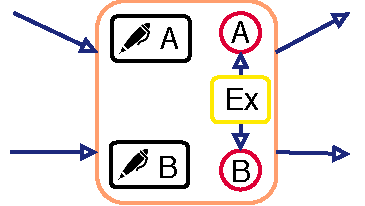
\includegraphics[width=0.8\textwidth]{images/exchange_block.pdf}
        \caption{Conceptual representation}
        \label{fig:exchange_block_conceptual}
    \end{subfigure}
    \begin{subfigure}{0.49\textwidth}
        \centering
        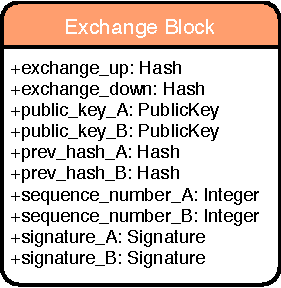
\includegraphics[width=0.6\textwidth]{images/exchange_block_data.pdf}
        \caption{Exchange block, data}
        \label{fig:exchange_block_data}
    \end{subfigure}
    \caption{A single exchange block for the TrustChain fabric. Source: \textit{Adpated from TU Delft BLockchain Lab}}
    \label{fig:exchange_block}
\end{figure}

Each agent keeps track of the actual set of blocks that were received in an exchange block such that 
the hash can be recalculated to check the validity of the exchange block. Specifically, each 
node stores an index of the blocks contained in an exchange in a separate database. This index can be 
used to retrieve the actual blocks from the database of blocks. This is illustrated in Figure \ref{fig:exchange_process}.

\begin{figure}
    \centering
    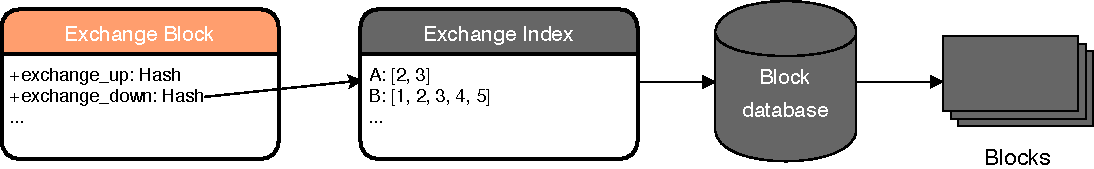
\includegraphics[width=\textwidth]{images/exchange_block_retrieval.pdf}
    \caption{Storage of exchange information: the exchange block contains a hash, which can be mapped to an index. That index can be used to retrieve the blocks from the block database.}
    \label{fig:exchange_process}
\end{figure}

\subsection{Exchange process}
We shall now describe the process of an exchange between two agents in detail. We consider two honest 
agents $A$ and $B$ in a Tribler context. $A$ would like to stream a video which $B$ possesses. According
to some exchange policy, $A$ is required to exchange information with $B$ and verify it before the 
interaction can take place. Thus, $A$ initiates the exchange by sending $A$'s complete chain to $B$,
together with a block index for each exchange block.
$B$ can perform simple checks on the chain, for example whether it contains the correct exchanges 
according to the exchange policy and whether all blocks are correctly signed and chained. From the 
chain and the exchange block indexes, $B$ is able to reconstruct the complete database index of $A$ which 
is the equivalent of the subjective network state from Section~\ref{sec:definitions}. 

At this point the action of $B$ depends on the actual exchange policy that is employed. According to
the Hisory-Exchange policy (see Section \ref{sec:model_double_spend}) $A$ has already provided 
enough information and $B$ will send his own chain. For the Network-State-Exchange policy it works as
follows. Given $A$'s database index, $B$ can calculate the difference between their databases. $B$ will 
then request from $A$ the blocks that $A$ has but $B$ does not. Once $A$ replies, $B$ has all 
information that $A$ has. $A$'s subjective network state has become transparent to $B$. We will refer
to this state later as subjective network state transparency.

$B$ is then able to recalculate all exchange hashes of $A$ to check that 
the exchange blocks are correct. If $A$'s chain completely checks out, $B$ sends his chain, exchange
indexes and blocks to $A$. Note that $B$ already knows which blocks $A$ is missing with respect to 
$B$ and can therefore directly send them. 

Now $A$ is able to perform the same checks as $B$. If $B$'s data also checks out, $A$ will create 
a new exchange block. The exchange block contains the root hash of the data that $A$ uploaded to $B$ 
and downloaded from $B$. As $B$ also knows that he downloaded from $A$ and uploaded to $A$, $B$ should
be able to calculate the same hashes. After both parties sign the block, they add them to their 
database of blocks. Also they create an entry for the exchange block in the exchange index map, which 
maps each exchange block to the index of exchanged blocks. Finally, they are able to perform the 
actual uploading and downloading of data. 

% \subsection{Obtaining a subject network state}
% One property of the extended architecture that we proposed in this section is that an agent's complete
% database is transparent to other nodes. It enables nodes to explore another node's view of the network. 
% In our model we called this the subjective network state. 

% Specifically, a node $A$ obtains a complete
% chain from an agent $B$ which includes transaction and exchange blocks. Furthermore, for each exchange 
% $B$ provides $A$ with the index of blocks contained in that exchange. If $A$ is able to recalculate 
% all the exchange hashes stored in the exchange blocks of $B$, $A$ has at least all information that 
% $B$ has and is able to obtain an exact similar subjective network state as $B$. If not, $A$ can see 
% from the exchange indexes which blocks $B$ has that $A$ does not. $A$ can request those from $B$, and
% if $B$ is honest $B$ will respond. Finally, 



\subsection{Scalability concerns}
Each exchange between agents adds an additional block to their chain. Also, the blocks that the 
exchange contains need to be transmitted and stored. This increases the bandwidth and storage 
requirements. However, the main property of linear scalability 
still applies, at least when assuming that storage capacity is not a problem. Each exchange and 
transaction still only requires two agents to communicate, thus parallel transactions are still 
possible and the example given in Section \ref{sec:trustchain_scalability} applies in the same way.
Problems occur when we include the storage requirement. For example, the Network-State-Exchange policy
requires agents to exchange all blocks with each transaction partner. Thus each agent that periodically
interacts will approach the complete network state. Depending on the agents transaction frequency and
the network's frequency there is a considerable delay between the subjective agent's state and the
network state. Still, this will lead to storage problems if agents need to run on personal computers
or even mobile devices.

% Exchange policies allow the system designer to ship software with a less or more stringent
% exchange policy. This will reduce or increase security but also impact the requirements on storage and bandwidth.
% If a stringent policy is applied, it should be possible to delete data. This could also be recorded on chain. As only the 
% root hash of the exchanges are stored on an agents chain, a delete block should be possible by 
% recording in a similar fashion without the need to remove blocks from the chain. Therefore chain 
% consistency is kept intact. How this should be implemented in detail and a security analysis will 
% be left for future research.

\section{Using exchange records}
In TrustChain the exchange behavior of agents was not visible. With the extended
architecture agents can base their decisions, for example whom to interact with, on how much data 
agents exchanged in the past. But making the gossiping behavior visible can only be the first step. 
The next step is naturally to apply the exchange records to work towards a safer distributed system.

In this section we explore ways of using the the exchange records. 

\subsection{Exchange policy flexibility}
The architecture that we have presented in the previous section is very flexible. Any size of information 
exchange between two parties can be recorded. It therefore allows for the implementation of any 
exchange policy. We have shown in Chapter \ref{chap:model} that the Network-State-Exchange policy
can give strong guarantees for security but also induces the highest cost on storage and bandwidth 
capacity. Depending on the application this might be necessary however TrustChain was designed to 
be as scalable as possible without global consensus. Therefore also less demanding exchange policies
can be implemented.  

\subsection{Attacks}
We now consider possible ways to attack the extended TrustChain system. 

\paragraph{Block tampering}
Similar to the block tampering that we described in Section \ref{sec:tampering}, an agent could 
directly change the hash of received blocks after an exchange. Again, the signature of the partner 
stored in the block will be invalidated. 

\paragraph{No actually storing information}
The information that is received is only recorded in form of the root hash of contained blocks. The 
actual blocks are in the database of the agent itself which is obviously opaque to other agents. 
Therefore an agent $A$ could possible only record correctly the exchange but not actually store the 
received information. 

However, other agents are expecting $A$ to be in the possession of the block. Thus, depending 
on the exchange policy, an agent might at some point request a block in which case $A$ is not able 
to respond. This will expose the agent of free-riding on the storage.

% \paragraph{Collusion}
% As we have previously discussed in Section \ref{sec:collusion}, attacking agents can work together in 
% a collusion attack. We claim that a subset of those collusion attacks is more difficult if agents are
% able to obtain subjective network state transparency. Consider two agents $A$ and $B$ are colluding 
% in a block tampering. $B$ has changed a block in order to obtain more reputation and $A$ is transacting 
% with $B$ to receive some of the maliciously gained reputation. But in order to transact and be considered
% an honest agent, $B$ needs to obtain $A$'s chain. In that case 

\subsection{System level trust}
\label{sec:system_trust}
Instead of enforcing a certain policy, the exchange records can also be used to create a system level 
notion of trust. We have extensively introduced the concept of trust in Chapter~\ref{chap:introduction} and discussed
how it plays a role in different contextual settings. Afterwards we have mostly considered trust in 
an application context like Tribler. TrustChain records transactions between users in the application
context which act as evidence of a user history. That history is used to calculate a reputation and
ultimately a trust value for each known user. Yet, the architecture of TrustChain and even more so 
the architecture of the extended TrustChain make room for another concept of trust on a system level.

Each agent in the system engages in recording, exchanging and verifying behavior. Agents do this 
with a certain reliability. Until now we assumed that agents are either perfectly honest, malicious
or free-riders, so there was no forgiveness and no shades of honesty. That is fine when considering
automated agents in a theoretical setting, however in practice this may not be realistic or 
desired. Instead we could assign a reputation to agents based on their exchange and verification 
behavior which is increased with ``positive'' action like exchanges and decreased with any 
``negative'' evidence, like multiple interactions without exchanges. Also, if we consider the way 
we defend against verification free-rider as described in Section \ref{sec:verification_free-riding}, 
agent completely redo all verification of an agent in order to verify that the agent behaved correctly.
Trust at system level could create a relationship between agents such that they can rely on each 
other's verification of peers. 

\section{Example}
In order to make the implementation more clear, an example is provided in this section. We look at two
agents, Alice and Bob. Both agents use the Network-State-Exchang policy, that is all knowledge is 
exchanged. Alice wants to interact with Bob and starts the interaction. We assume that
both agents are new to the network and only have their genesis blocks on the chain. In order to
start the interaction, Alice sends her chain (only the genesis block) and an empty set of exchanges
to Bob. Obviously the genesis block is accepted and Bob shows his approval by sending his own
genesis block and an empty set of exchanges. Also Alice accepts the data. Alice creates an exchange
block which includes in the field \verb|exchange_up| the hash of Alice's genesis block and in the field 
\verb|exchange_down| the hash of Bob's genesis block. Alice signs that block and sends it to Bob. 
Bob verifies that the hashes actually are correct. If Bob agrees, he also signs the block and returns 
it to Alice. Alice also stores an block index for the created exchange block which includes as entry 
only Bob's block with sequence number 1. Similarly, Bob documents that he received Alice's first block
in the new exchange block.

At this point both agents are sure that they are honest and are able to interact in the 
application context. For example, Alice could not stream a video from Bob. After the transaction in 
the application context, Alice creates and signs a transaction block and sends it to Bob who replies 
in a similar fashion if he agrees. Figure \ref{fig:exchange_example} shows the chains of Alice and Bob after the complete interaction. 

\begin{figure}
    \centering
    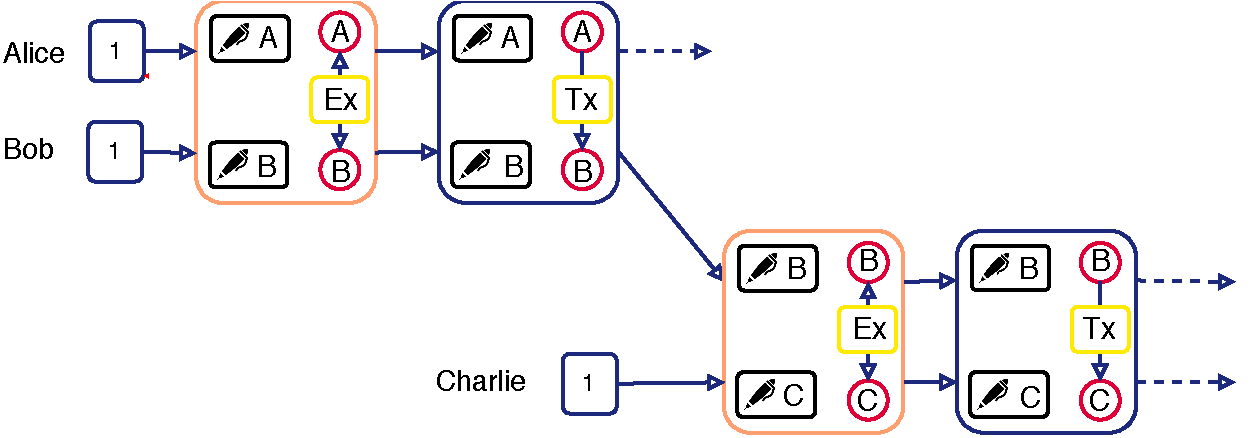
\includegraphics[width=\textwidth]{images/trustchain_example.pdf}
    \caption{Example of three agents interacting}
    \label{fig:exchange_example}
\end{figure}

This example sheds light on the block creation process but is too simple to properly explain the 
exchange and verification process. We extend the example with another agent, Charles, whom Bob would
like to interact with after the previous interactions. Again, Charles is assumed to be new to the 
network so the genesis block is the only block on his chain. Bob starts the interactions by sending
his chain and the index that documents the acquisition of Alice's first block. 

Charles sees that Bob has an exchange block with Alice before have a transaction with her, which is 
correct according to the exchange policy. Next Charles checks the signatures and hashes of Bob's chain. 
After those checks pass, Charles tries to calculate the hashes for Bob's exchange block but realizes
that he does not have Alice's first block. Therefore he requests it from Bob. After receiving it the
check should pass. 

Once Charlie accepts all the checks, he sends his own chain and exchanges which are checked by Bob
and the interaction continues as previously described. Table \ref{tab:blocks_example} shows the
blocks that each agent has after the first and second round. After the second round, Charles has 
all the blocks from Bob that he had after the first round.

\begin{table}[h!]
    \centering
    \caption{The block databases of each agent for the example}
    \label{tab:blocks_example}
    \begin{tabular}{p{4cm}|p{3cm}|p{4cm}|p{3cm}}
        \toprule
        Database & Alice & Bob & Charles \\
        \midrule
        Before first round & A: $[1]$ & B: $[1]$ & C: $[1]$ \\ \hline 
        After first round & A: $[1, 2, 3]$ \newline B: $[1, 2, 3]$ & A: $[1, 2, 3]$ \newline B: $[1, 2, 3]$ & C: $[1]$ \\ \hline
        After second round &  A: $[1, 2, 3]$ \newline B: $[1, 2, 3]$ & A: $[1, 2, 3]$ \newline B: $[1, 2, 3, 4, 5]$ \newline C: $[1, 2, 3]$ & A: $[1, 2, 3]$ \newline B: $[1, 2, 3, 4, 5]$ \newline C: $[1, 2, 3]$ \\
        \bottomrule
    \end{tabular}
\end{table}

% * Verification and exchanges make an agent trustworthy on a system level, as in, we trust them to 
% stick to the rules of recording, exchanging and verifying
% * Use this to not verify each and every agent, but assume agent which were verified by trustworthy
% agents to be trustworthy enough for interaction
% * At every point we still have the chance to do the complete verification of a history. But maybe 
% its not required every turn